\chapter{Single Photon Emission\\Computed Tomography (SPECT)}
\vspace{-45ex}
\begin{flushright}
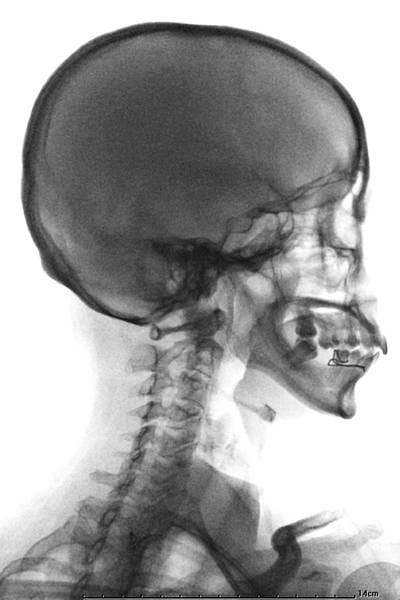
\includegraphics[width=4.5cm]{SPECT_example} % https://www.cidrad.com/wp-content/uploads/2024/06/testicular-ultrasound-riverside-county-ca-usa-near-me-400-600.jpg
\end{flushright}

\section{Acquisition}
\begin{itemize}
\item \gls{SPECT} is the tomographic counterpart of nuclear medicine
  planar imaging, just like CT is the tomographic counterpart of
  radiography.
  
\item In SPECT, a nuclear camera records X- or Gamma-ray emissions
  from the patient from a series of different angles around the
  patient.
  
\item  These projection data are used to reconstruct a series of
  tomographic emission images.
\end{itemize}

\section{Clinical applications}
\begin{itemize}
\item SPECT images provide diagnostic functional information similar
  to nuclear planar examinations; how- ever, their tomographic nature
  allows physicians to better understand the precise distribution of
  the radioactive agent, and to make a better assessment of the
  function of specific organs or tissues within the body.
\item The same radioactive isotopes are used in both planar nuclear
  imaging and SPECT \cite{bushberg2011essential}.
\end{itemize}
